\subsubsection{Estensione D: Mancata Connessione al Sistema}

In alcune circostanze, il manager potrebbe non riuscire a completare la registrazione a causa di problemi di connessione o di un temporaneo malfunzionamento del server.
Il sistema gestisce questa evenienza fornendo un chiaro feedback sull’esito negativo dell’operazione.

\subsubsection{Gestione dell’Errore di Connessione}
Dopo aver cliccato su \textbf{“Conferma”}, il sistema mostra un breve stato di caricamento.
Se la connessione al server non riesce, viene visualizzato un pop-up di allerta che informa l’utente dell’impossibilità di completare la registrazione per motivi tecnici.

In questo caso, l’\textbf{use case è considerato fallito}, ma il manager può chiudere il messaggio e riprovare l’operazione una volta ristabilita la connessione.
Questa soluzione si basa sui principi di \textbf{visibilità dello stato del sistema} e di \textbf{recuperabilità dall’errore}, assicurando chiarezza e prevedibilità anche in situazioni di errore tecnico.
\begin{figure}[H]
	\centering
	\begin{tikzpicture}[node distance=1.5cm and 1cm, auto]
			% Nodo per immagine 3 con didascalia sotto, posizionato sotto img2
		\node (img1){
			\begin{tabular}{c}
				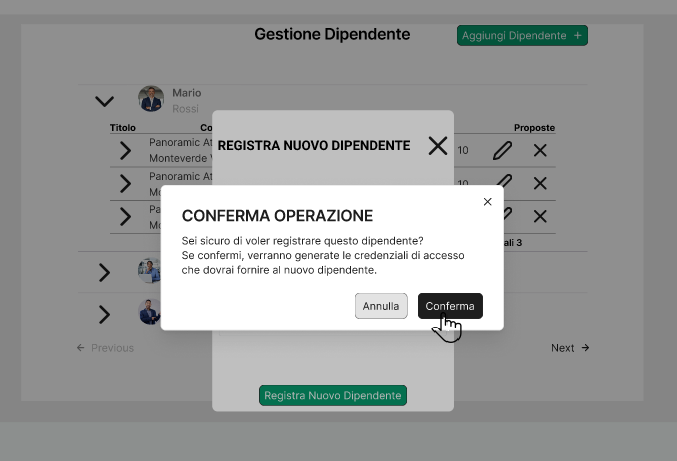
\includegraphics[width=0.7\textwidth]{Immagini/Mockup/nuovoAgente/scenario principale/ClickAllertConferma.png} \\
				Cockburn: step 6.D
			\end{tabular}
		};
		
		% Nodo per immagine 1 con didascalia sotto
		\node (img2)  [below=of img1] {
			\begin{tabular}{c}
				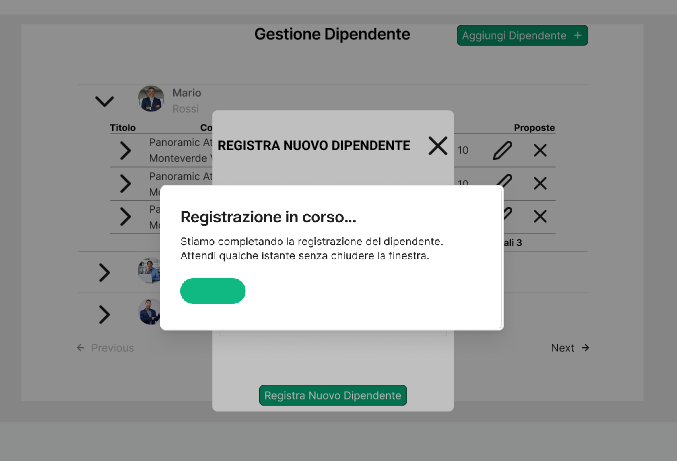
\includegraphics[width=0.7\textwidth]{Immagini/Mockup/nuovoAgente/scenario principale/caricamentoRegistrazione.png} \\
				Cockburn: step 7.D
			\end{tabular}
		};
		
		% Nodo per immagine 3 con didascalia sotto, posizionato sotto img2
		\node (img3) [below=of img2] {
			\begin{tabular}{c}
				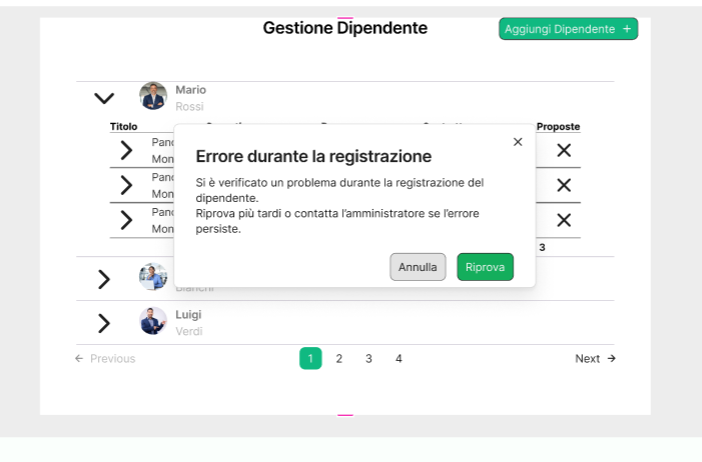
\includegraphics[width=0.7\textwidth]{Immagini/Mockup/nuovoAgente/extension D/messaggioDiErrore.png} \\
				Cockburn: step 8.D
			\end{tabular}
		};
		
		% Disegna le frecce
		\draw[->, thick] (img1) -- (img2);
		\draw[->, thick] (img2) -- (img3);
		
	\end{tikzpicture}
	\caption{Mockup: Extension D della tabella di Cockburn del caso d'uso: Registra nuovo agente.}
	\label{fig:tikz_flow}
\end{figure}